\newsection
\subsection{Theory}
\label{sec:theory}
\sectionauthors{Aditi Raghunathan, Sang Michael Xie, Ananya Kumar, Niladri Chatterji, Rohan Taori, Tatsunori Hashimoto, Tengyu Ma}

\newcommand\lpre{\ensuremath {\ell_{\text{pre}}}}
\newcommand\emppre{\ensuremath {\widehat{L}_{\text{pre}}}}
\newcommand\popadapt{\ensuremath {L_{\text{adapt}}}}
\newcommand\empadapt{\ensuremath {\widehat{L}_{\text{adapt}}}}
\newcommand\poppre{\ensuremath {L_{\text{pre}}}}
\newcommand\datapre{\ensuremath {p_{\text{pre}}}}
\newcommand\trainpre{\ensuremath {\hat{p}_{\text{pre}}}}
\newcommand\datatask{\ensuremath {p_{\text{task}}}}
\newcommand\traintask{\ensuremath {\hat{p}_{\text{task}}}}
\newcommand\thetaum{\ensuremath {\hat{\theta}_{\textup{FM}}}}
\newcommand\gammatask{\ensuremath {\gamma_{\text{task}}}}
\newcommand\ladapt{\ensuremath {\ell_{\text{adapt}}}}
\newcommand\poptest{\ensuremath {L_\text{task}}}

Rigorous mathematical theory plays a foundational role in many engineering and science disciplines (\eg information theory in electrical engineering). We believe that theory of foundation models can be particularly beneficial in guiding technical decisions and innovations because of the huge computational costs associated with experimenting on foundation models. 
In addition, theoretical insights help elucidate fundamental limitations and explain surprising empirical phenomena.
However, the community currently has a limited theoretical understanding of foundation models, despite much recent progress~\cite{arora2019theoretical,haochen2021spectral,wei2021pretrained,wei2020theoretical,zhang2021inductive,saunshi2020mathematical,dao2019kernel,tosh2020contrastive,tosh2021contrastive,cai2021theory,lee2020predicting,zimmermann2021contrastive,bansal2020self,wang2020understanding,tsai2020self,tian2020makes,tian2020understanding, tripuraneni2020theory,du2020fewshot}. 

Deep neural networks form the backbone of foundation models. 
Even in the well-studied supervised learning setting, where the train and test scenarios have the same distribution, there are numerous open questions around deep nets such as understanding non-convex optimization, the implicit regularization effect of optimizers, and expressivity. Foundation models raise questions that significantly go beyond the supervised deep learning setting. 
The core problem in theoretically analyzing foundation models is understanding why training on one distribution with a possibly unsupervised/self-supervised loss leads to good adaptation performance on \emph{different} downstream distributions and tasks.\footnote{The theory for foundation models closely relates to, but also goes beyond the theory for transfer learning (which is itself an underexplored area): foundation models are possibly trained with unlabeled data and will be adapted to many or all natural tasks, whereas transfer learning typically studies labeled source tasks and a fixed number of target tasks.}

We will discuss an intuitive modularization to analyze foundation models that lays bare the connections between supervised learning and foundation models, concrete and core technical questions, and some promising theoretical tools to address these questions. These new core questions can provide useful insight into foundation models and can be studied in parallel to supervised deep learning theory. While we focus on analyzing the downstream performance, the proposed modularization and tools could prove useful to analyze other metrics of interest such as robustness to distribution shifts (\refsec{robustness}) and security (\refsec{security}).

\begin{figure}[!ht]
\centering
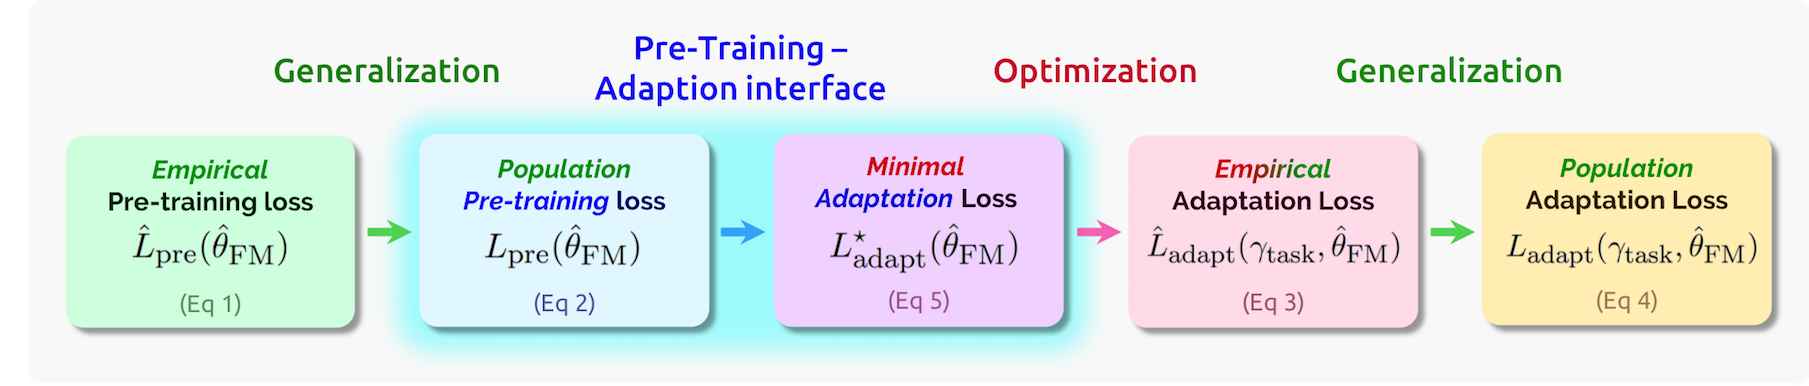
\includegraphics[width=\linewidth]{technology/figures/Theory.png}
\caption{\label{fig:theory} The analysis of foundation models from pretraining on diverse data to downstream performance on adapted tasks involves capturing the relation between different loss terms as shown above. The main challenge is to analyze the highlighted pretraining-adaptation interface which requires reasoning carefully about the population losses in addition to the model architecture, losses and data distributions of the pretraining and adaptation stages (\refsec{theory-interface}). Analysis of generalization and optimization largely reduces to their analysis in standard supervised learning.}
\end{figure}

\subsubsection{Theoretical formulations and modularizations}
\label{sec:theory-modularizations}
Recall that foundation models are trained on a large amount of raw data (\refsec{training})  then adapted to specific tasks (\refsec{adaptation}) and therefore can be decomposed naturally into training and adaptation phases. We identify interfaces between them and disentangle parts specific to foundation models from parts that require standard deep learning theory, so that they can be independently worked on. We introduce a modularized analysis framework, which has also been implicitly or explicitly employed in recent works, \eg~\citet{arora2019theoretical,haochen2021spectral,wei2020theoretical,tripuraneni2020theory}. The crucial component in this modularized analysis turns out to be the \emph{pretrain-adaptation interface.} We first describe the modularization, and discuss why we find this modularization promising and finally some limitations. 

We will refer to the training phase explicitly as ``pretraining'' to distinguish it from the adaptation phase that could also involve training on a few samples from a particular task. 

\paragraph{Pretraining phase.} 
The pretraining of foundation models often involves a data distribution $\datapre$ (\eg the distribution of natural text) and a \emph{pretraining loss} function $\lpre(x;\theta)$ that measures the loss (\eg language modeling loss in GPT-3) on an input $x$ for a model with parameters $\theta\in \Theta$. Let $\trainpre$ denote the empirical distribution over a large number of independent samples from $\datapre$. 

Pretraining minimizes the loss $\lpre$ on $\trainpre$, which we call \textit{the empirical pretraining loss}, and produces a model $\thetaum$:
\begin{align}
    \emppre(\theta) \eqdef \E_{x\sim \trainpre}[\lpre(x;\theta)],
        ~~\text{and}~~
\thetaum \eqdef \argmin \limits_{\theta \in \Theta} \emppre(\theta).
\end{align}

We consider the corresponding loss on the population distribution $\datapre$, called the \textit{population pretraining loss}, as a central concept: 
\begin{align}
   \poppre(\theta) \eqdef \E_{x\sim\datapre}[ \lpre(x; \theta)] .
\end{align}

\paragraph{Optimization-based adaptation phase.} 
We frame adaptation as a general constrained optimization problem that depends on $\thetaum{}$, abstracting away those adaptation methods that are based on optimizing certain loss functions such as fine-tuning and prompt-tuning (see, \eg ~\citep{houlsby19adapter,li2021prefix,lester2021power}, and \refsec{adaptation}).

Since different adaptation methods could modify different subsets of the model parameters, we denote the space of adapted model parameters by some $\Gamma$. Given a downstream task distribution $\datatask$ (\eg question answering in a particular domain) and a few empirical samples $\traintask$ sampled from $\datatask$, we model the adaptation phase as minimizing some \textit{adaptation loss} $\ladapt$ on $\traintask$ w.r.t adapted parameters $\gamma \in \Gamma$: 
\begin{align}
\gammatask(\thetaum) \eqdef \argmin \limits_{\gamma \in \Gamma, C(\gamma;\thetaum)\le c_0 }\empadapt(\gamma, \thetaum),
\end{align}
where $\empadapt(\gamma, \thetaum) \eqdef \E_{x\sim \traintask}[\ladapt(x;\gamma, \thetaum)]$ is the empirical adaptation loss, and $C(\gamma, \thetaum)\leq c_0$ is an optional constraint that controls the complexity of the adapted parameters, encompassing both explicit regularization (\eg model dimensionality and norm) and the implicit regularization of the adaptation process. 

We list some common adaptation methods and discuss the corresponding adapted parameter $\gamma$ and constraints $C(\gamma, \thetaum)\leq c_0$. 
\begin{enumerate}
    \item Linear probing: training a linear classifier on top of the representations from a foundation model. Here $\Gamma = \R^k$ is the set of linear classifiers on the representations of dimensionality $k$, and $C(\gamma, \thetaum)$ could be the $\ell_2$ or $\ell_1$ norm of $\gamma$. 
    \item Fine-tuning: optimizing a randomly initialized linear head for a few steps, and all other parameters $\theta$ from the initialization of $\thetaum$. Here $\gamma$ is the concatenation of $\theta$ and the linear head. Such a process could correspond to some implicit regularization of $\gamma$ towards the initialization $\thetaum$ captured by $C(\gamma, \thetaum) \leq c_0$. The exact term $C(\gamma, \thetaum)$ would depend on the optimization algorithm used, and such a characterization of the implicit regularization of optimization is an area of active research study ~\citep[\eg][and references therein]{gunasekar2017implicit, soudry2018implicit,gunasekar2018implicit,arora2019implicit, blanc2019implicit,woodworth2020kernel, wei2020implicit, haochen2021shape,damian2021label}.\footnote{
    It may not always be feasible to characterize the inductive bias of adaptation via an explicit constraint $C(\gamma,\thetaum)\leq c_0$. The modularization we propose is also applicable in these cases, but for notational simplicity, we focus on the case where implicit regularization can be approximated via an explicit constraint.
    }
    \item Prompt-tuning: optimizing a small set of continuous task-specific vectors that prepend the task inputs. Here $\gamma$ is the continuous prompt vectors which often has small dimensionality, and we may optionally have a constraint on the norms of $\gamma$. 
\end{enumerate}

One obvious limitation to note is that this formulation excludes adaptation methods such as in-context learning~\citep{brown2020gpt3} where there is no ``training'' (\ie the minimization of some empirical adaptation loss) during the adaptation phase. We discuss this and other limitations in \refsec{theory-incontext}. 

Two central quantities for the adaptation phase are the \textit{population adaptation loss}
\begin{align}
    \popadapt(\gamma, \thetaum) = \E_{x\sim\datatask}[ \ladapt(x; \gamma,\thetaum)]
\end{align}
and the \emph{minimal adaptation loss} 
\begin{align}
    \popadapt^\star(\thetaum) = \min_{\gamma \in \Gamma, C(\gamma;\thetaum)\le c_0}\popadapt(\gamma, \thetaum)
    \label{eqn:5}
\end{align}

\paragraph{Separate analysis for modularized phases.} Existing generalization theory for standard supervised learning aims to show that $\emppre\approx \poppre$ and $\empadapt\approx \popadapt$. 
Addressing these questions specifically for deep nets is an active research area. 
We can also leverage the standard learning theory decomposition to bound the final downstream task loss by the excess generalization error and the minimal adaptation loss as follows. 
 \begin{align}
    \popadapt(\gammatask, \thetaum) \le \underbrace{\popadapt^\star(\thetaum)}_{\textup{minimal adaptation loss}} + \textup{~~generalization error}
    \label{eqn:6}
\end{align}
where the generalization error captures the closeness between $\popadapt$ and $\empadapt$.\footnote{More precisely, the generalization error term is the sum of  $\popadapt(\gammatask, \thetaum) -  \empadapt(\gammatask, \thetaum)$ and $\empadapt(\gammatask^\star, \thetaum)-\popadapt(\gamma^\star, \thetaum) = \empadapt(\gammatask^\star, \thetaum)-\popadapt^\star(\thetaum)$, where $\gammatask^\star$ is the minimizer of \refeqn{5}. \refeqn{6} follows easily be using $\empadapt(\gammatask, \thetaum)\le \empadapt(\gammatask^\star, \thetaum)$.}
The decomposition and relationship between these key quantities are shown in \reffig{theory}. 
The generalization and optimization arrows, as argued above, largely reduce to deep learning theory in the supervised setting. 
What we are left with is the main challenge with foundation models, which is to understand why the minimal adaptation loss $\popadapt^*(\thetaum)$ can be small as a result of a small pretraining population loss, which we dive into next in \refsec{theory-interface}.

The work of~\citet{arora2019theoretical} pioneered the pursuit of this question by bounding from above $\popadapt^\star(\thetaum)$ by $\poppre(\thetaum)$ in the context of contrastive learning, and ~\citet{haochen2021spectral,tosh2020contrastive,tosh2021contrastive} relax the data assumptions. Other pretraining methods successfully analyzed under this framework (implicitly or explicitly) include pretraining with language models ~\cite{wei2021pretrained} or self-supervision~\cite{lee2020predicting}, with self-training algorithms~\cite{wei2020theoretical,cai2021theory}, and with multiple supervised tasks ~\cite{tripuraneni2020theory,du2020fewshot}. 

\subsubsection{Why is the pretraining-adaptation interface interesting?.}
\label{sec:theory-interface}
As shown in \reffig{theory}, the main missing link beyond standard supervised theory is:
\begin{center}
    \emph{Under what conditions does a small population pretraining loss $\poppre(\thetaum)$ imply a small minimal adaptation loss $\popadapt^\star(\thetaum)$} and why?
\end{center}
The conditions that lead to a successful interface could depend on several quantities such as the pretraining and adaptation distributions, objectives and training methods, as well as the model architecture. This question is beyond the scope of standard generalization theory, but it does narrow us down to a few important factors specific to foundation models, and captures the essence of various important open questions on foundation models as we argue below.  

First, we note that this interface deals with population quantities that concern two \emph{different distributions}. Hence, the conditions for a successful interface are likely to involve special properties of the distributions, for example, the diversity of the pretraining distribution and structural shifts between the pretraining and adaptation data. This makes the analysis of the interface challenging (as discussed below in \refsec{theory-tools}) as we need to make careful modeling assumptions about how the two distributions relate to one another. However, this presents the possibility that tools and techniques developed to analyze such interfaces could be useful to understand the effect of distribution shifts and to predict when foundation models can improve robustness. 

Second, the population losses and possibly the conditions of a successful interface depend on the \emph{model architecture}. This raises the challenge of opening up the black-box of the neural nets. What does a small pretraining loss on a particular distribution tell us about the properties of the intermediate layers? Such analyses would also guide us in designing new adaptation methods that more carefully exploit different intermediate representations. 

Third, \emph{few-shot learning} or the sample efficiency of adaptation can be captured through the constraint on the complexity measure $C(\gamma, \thetaum) <c_0$ in the minimal adaptation loss. 
We need to formally characterize these complexity measures (\eg by understanding the implicit regularization effect of the adaptation process) and further understand why a small population pretraining loss would imply a low-complexity adaptation parameters $\gammatask$. 
A satisfactory answer to this question would likely allow us to improve the sample-efficiency of downstream adaptation.

Finally, and importantly, critical components of the interface are the choice of the \emph{pretraining and adaptation losses}. We want to understand how to best combine the pretraining and adaptation objectives for successful adaptation. It is possible that the pretraining objective that best guarantees successful adaptation differs from what is explicitly minimized during the pretraining process\dash{}the interface above allows one to use any surrogate population objective on the pretraining distribution. In addition, new surrogate objectives that provably lead to good adaptation across a broad set of tasks could shed light on the fundamental aspects that make foundation models successful. 

To summarize, the interface precludes the issue of generalization and allows us to formally reason about the interaction between several important quantities of the pretraining and adaptation phases that can guide practice in important ways.

\subsubsection{Challenge: analysis of in-context learning and other emergent behavior}
\label{sec:theory-incontext}
GPT-3~\citep{brown2020gpt3} demonstrates the power of in-context learning, an adaptation method that does not need any parameter optimization. In the adaptation phase, the pretrained language foundation model takes in a prompt\dash{}a sequence of tokens that concatenates input-output examples from the task\dash{}followed by a test example and simply generates the label of the test example by conditioning on the sequence seen thus far (prompt plus test example). 
In other words, there is no explicit training or change to the model parameters.  
What is the mechanism by which the model ``learns'' from the different examples by simply executing with the examples as inputs?
The previous modularization does not directly apply because we do not obtain new model parameters during adaptation, but rather we only use the generative capabilities of the foundation model by executing on structurally-designed inputs. 
More broadly, the proposed modularization provides a nice framework to gain useful theoretical insights into foundation models as discussed above. But it is possible that some emergent behavior like in-context learning and other capabilities yet to be discovered would require going beyond the modularization.

\subsubsection{Challenge: appropriate data assumptions and mathematical tools.}
 \label{sec:theory-tools}
Understanding the interface between pretraining and adaptation phases requires a more careful study of data distributions than in traditional supervised learning. This is because the pretraining and task adaptation distributions are inherently different. By definition, foundation models are trained on raw data that is typically extremely diverse and task-agnostic, while the adaptation data depends  heavily on the task. Similarly, in-context learning emerges as a result of learning to generate data that looks like the pretraining distribution, and thereby understanding in-context learning requires careful modeling of the pretraining data. Hence answering the central questions around foundation models requires realistic and interpretable assumptions that are also amenable to analysis. 
Recent works either assume certain properties of the population data, \eg the expansion property in \citet{haochen2021spectral, wei2020theoretical}, or that the population data is generated from latent variable models with some structure~\citep{SaMa20mat,wei2021pretrained,arora2015latent,lee2020predicting,zhang20ont,tosh2021contrastive}.


We generally lack mathematical tools for relating properties of foundation models to the structure in the population data distribution.  ~\citet{haochen2021spectral} applies spectral graph theory to leverage the inner-class connectivity in the population distribution. More precise characterization of $\thetaum$ via probabilistic and analytical derivations is possible for latent variable models, but so far restricted to relatively simple ones. The community will significantly benefit from more systematic and general mathematical tools to address this question. 

It is also highly desirable to define simple toy cases so that theoreticians can precisely compare the strengths of various tools and analyses. For example, \citet{haochen2021spectral} and \citet{wei2020theoretical} consider the mixture of manifolds problem which might potentially be a good simplified test bed for vision applications. We need more interesting test beds for discrete domains such as NLP. 
We believe that tractable theoretical models which capture relevant properties of real datasets are a crucial step towards placing foundation models on solid theoretical footing.